%File: introduction.tex
%Date: Sat Oct 19 13:39:05 2013 +0800
%Author: Yuxin Wu <ppwwyyxxc@gmail.com>

\section{Introduction}
\subsection{Background}
The use of social networks spread rapidly.
It became a common sense that information is collected through online information portal.
This product mainly aims to help users collect useful information
as well as manage their personal information in convenience.

\subsubsection{Complexity of Information Resources}

    Nowadays there are various sources of information.
    Light-weight sources, such as RenRen, Sina Micro Blog (Weibo) produce
    news all the time. An ordinary user would use many of them,
    then he needs to open several different web pages, or different phone applications,
    in order to get all the news feeds.

    Moreover, those heavy-weight sources like NetEase, Yahoo!,
    or individual blogs may produce information from time to time.
    Readers may not be willing to consecutively refresh them to get the latest article,
    which will be both time-consuming and bandwidth-consuming.

    According to the pre-survey we made,
    most social network users are facing this situation that the complexity
    of information resources is causing them problems.

\begin{description}
  \item[Quantity] \hfill

    The large quantity of web portals,
    social networks makes users tired of changing and choosing between web pages or applications.
    Users tend to only focus on specific types of information, but will suffer from the large quantity of
    the information presented to them.

  \item[Redundancy] \hfill

   It is a waste of time for users to acquire similar information through different portals.
   Users is long for a tool to automatically, intelligently filter the repeated information from different
   sources.

\end{description}

   Therefore, an information collector with corresponding filter is in great demand,
   in order to simplify the flow of getting the latest information.
   Users can browse their favourite for one time in just one place.

   It is an obvious conclusion that users are in badly needed to one browsing-friendly
   page that simply contains all and exactly all the information they need.

\subsubsection{Analysis of Existing Information Portals}
In this section, the possibility of combining information resources will be illustrated.
Let’s first take Sina Weibo\footnote{\url{http://weibo.com}}, Renren\footnote{\url{http://renren.com}} and
Zhihu\footnote{\url{http://zhihu.com}}, which are three major information sources of different types,
as examples.

\begin{enumerate}
  \item User Interface

It is not hard to find out that the user interfaces
designed by different websites do not distinguish each other too much.
There are considerably parts that follow certain similar format.
The interfaces are mainly divided into four categories:
\begin{enumerate}
  \item main interfaces
  \item personal interface
  \item managing and editing interface
  \item other individual functions
\end{enumerate}

\item Main Interface

    The main interface is the page that provides the most significant
    and useful information.
    Users mainly receive information through this page, therefore it is the
    information sources we should be working on.

    As we can see in the following figures, the main interfaces’ features are listed as followed:

\begin{figure}[H]
  \centering
  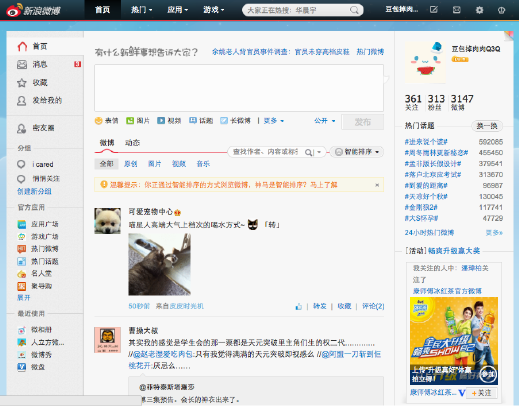
\includegraphics[width=0.8\textwidth]{img/weibo.png}
  \caption{Main Interface of Sina Weibo\label{fig:weibo}}
\end{figure}

\begin{figure}[H]
  \centering
  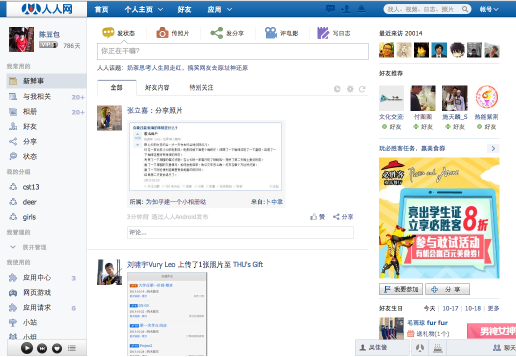
\includegraphics[width=0.8\textwidth]{img/renren.png}
  \caption{Main Interface of Renren\label{fig:renren}}
\end{figure}

\begin{figure}[H]
  \centering
  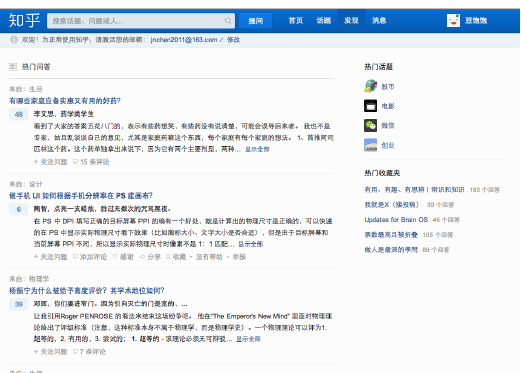
\includegraphics[width=0.8\textwidth]{img/zhihu.png}
  \caption{Main Interface of Zhihu\label{fig:zhihu}}
\end{figure}


\begin{enumerate}
  \item  Information items are listed and presented by vertical blocks. \figref{weibo}, \figref{renren}, \figref{zhihu}

  \item The item-block consists of the author, the subtitle, the content and the picture part. \figref{weibo}, \figref{renren}
\end{enumerate}

    Since the speciality of the format
    that the interfaces are following can be easily caught,
    it provides the great possibility to combine those pages together.

\end{enumerate}

\subsection{Purposes}
    Uknow InfoHub is designed according to the needs of users.
    It will provide users with a entirely new experience in gathering information --
    by using only one information collector.
    Technically, a collector which can be customized and
    widened is required, for it's inevitable that different users ask for
    different classification information.
    Even more, if the collector contains a recommendation system, which can be capable to suggest subscribers
    articles they may interested in, users will be more sticky to
    this collector in all probability.

    \subsection{Future Works}

 Uknow InfoHub shall provide extensible interfaces.
 The Open API makes it possible to expand different functions based on this collector.

 For instance, a Text-to-Speech system can be used upon the collector, so that
 users will be able to hear the information instead of browsing.
 Meanwhile, based on the users behavior, a recommendation system could be most valuable
 to users that recommend stuff which is meaningful to individual users. An Ad-targeting system
 can also be built directly on this.

 This collector should provide the easy functionality to be used
 on various operating systems as well as various devices, such as Android, iOS, Linux, Windows.
